\documentclass[10pt,conference]{IEEEtran}
\usepackage{cite}
\usepackage{amsmath,amssymb,amsfonts}
\usepackage{algorithmic}
\usepackage{graphicx}
\usepackage{textcomp}
\usepackage{xcolor}
\usepackage[]{algorithm2e}
\def\BibTeX{{\rm B\kern-.05em{\sc i\kern-.025em b}\kern-.08em
    T\kern-.1667em\lower.7ex\hbox{E}\kern-.125emX}}
\begin{document}

\title{Applying Supply Chain Management in Software Engineering Research: Opportunities and Challenges}
\author{\IEEEauthorblockN{Anonymous Authors \\
\textit{Authors' Affiliation}\\
City, State \\
authors@institution.edu}}

%\author{\IEEEauthorblockN{Krishna Prasad Neupane \\
%\textit{Rochester Institute of Technology}\\
%New York, USA \\
%kpn3569@rit.edu}
%\and
%\IEEEauthorblockN{Yi Wang \\
%New York, USA \\
%yi.wang@rit.edu}
%}

\maketitle

\begin{abstract}
A modern software development project relies on many libraries, APIs, and other types of artifacts developed by other projects. These project together form complex supplier and consumer relationships. This complexity raises many potential risks and unpredictability. Though SE is still in its early age to deal with this complexity, researchers in management have developed solid knowledge and grown a mature subarea--supply chain management. In this paper, we explore the possibility of applying supply chain management knowledge to software engineering research domain to address the complex supplier and consumer relationships between software projects. We demonstrate the
feasibility of this research direction with a preliminary case study on iPython--a high-profile interactive data analysis and visualization project. Our results show that using supply chain management models and techniques can help us to identify... We further summarize the opportunities and challenges. 


\end{abstract}

\begin{IEEEkeywords}
Supply chain management, iPython, risk                                                                      
\end{IEEEkeywords}

\section{Introduction--1 page}
To fulfill the user requirements, a developer must deliver high quality, robust and error-free software products within the limited budget\cite{sofCom}. However, the modern software project is greatly concerned about security and reliability; there is still a lack of risk analysis in a dependency network of a software project. The paper investigates risk in the dependency network with the help of industrial process-the supply chain. The supply chain system provides a supply-demand relationship between different dependency tiers and does coordination of information flow between linked dependencies in the network.

The supply chain risk analysis utilizes dependency packages of a software project to create a dependent matrices and then examines to figure out critical packages that cause higher risk in the project. The network of the supply chain includes a different layer of supply tiers and that assist to compute risk percentage in the different tier of the supply chain network.

The motivation behind this paper is exploiting supply and demand concept of well known industrial approach which provides efficient risk analysis for the dependency graph. The supply chain analysis provides risk parameters: number of dependencies, release date and release version for each package, so that it helps developer to decide whether particular network and package are becoming critical in the project or not. 

This paper attempts to analyze the risk of supply chain dependency network in a software project; exploiting a generic industrial concept called the supply chain. This novel approach is helpful for developers to figure out how critical the supply chain network is in the software project and also to measure the percentage of risk in different layers of software dependency tier.     

The paper is organized by providing brief background of key components and then methodology, evaluation and followed by the conclusion.

\section{Supply Chain Management in Software Engineering--0.75 page}
To make basic understanding of the key terminologies, we describe supply chain management and its important in the field of the software engineering.
\subsection{Supply Chain Management}
The term supply chain was introduced in 1982 by Oliver and Weber and they describe it as a "network of organizations that directly involves in the upstream and downstream flows of products\cite{} (ellram 1991)." The objective of the supply chain management is to balance the demand and supply in the supply chain network. The supply chain activities starts from the raw materials and extends all the way to the final customers. These activities include supplying raw materials, processing raw materials, making final products and then supplying final products to the customer. Each of these suppliers are working as a supply tier to its next tier. First tier of the supplier supplies final products to the customer while last tier supplier provides basic raw materials to the manufacturer. This chaining of the tier resembles supply chain in the industrial system.

An important aspect of the supply chain management is flow management\cite{}(steven book). Flow involves the movement of the product, sharing of forecast data, updating orders, providing payments and consignments. To manage the supply chain flow many industries integrate information technology and adopt lean principles in their supply chain management strategy. 


\subsection{Needs of Supply Chain in Software Engineering: Why it work?}
A typical oftware engineering project relies upon many external artifacts, e.g., libraries, packages, APIs, etc., to accomplish project goals. The project team, as a consumer, has very limited control on these external artifacts whose suppliers often do not have any overlap or connection with the project team. Thus, their relationships falls into classic supply chain management scenarios. For example...

%2 sentences state the problem.

Thus, applying the methods developed in supply chain management literature to solve the above problems is a very straightforward choice.
%give another example 2-3, how a problem may be solved.

The link between many libraries from own and other projects form the software supply chain in the software project development process. This supply chain concept can use to visualize in-depth interconnected and interdependent structure of the software project. This important aspect of the supply chain can use to manage risks and uncertainty of the flows between libraries. Usually supply is predicted on the basis of demand from consumer and depending upon the forecast done by management team, supply is provided to balance the consumer's demand. Similarly, in software project development this can predict more demanded libraries and then analyze its availability and risk associated in the chain. 


\subsection{Supply Chain features in Software Engineering: What it can offer?}
Supply chain management offers a systematic solution to many software engineering problems in a project's entire life cycle. In the requirement phase,. In the design phase, the decision-making on using which library can be analogized to the decision-making on selecting proper suppliers in SCM. In the implementation phase,...  

 The generic industrial supply chain concept coordinates between activities while producing goods and providing services. This concept provides similar perspective to the coordination required between multiple components of software project. Demand and supply requirement in the industrial model can be visualize as analogous concept to the dependency packages require for software project. This mechanism supports figuring out higher demanded packages in the project and critical path of the supply network. Dealing with these risk factors, supply chain tries to provide error-free, timely deliver, and cost effective demand supply balance for software project. 


\section{Case Study: Role of Supply Chain in IPython -- 1.5 page}
To demonstrate the potential of applying SCM in software engineering research, we conduct a case study on a popular open source software project--IPython. The case study, though in its preliminary stage, shows the promising scope of supply chain in the software engineering domain.


$RQ : show why supply chain is important at \\all in software engineering domain$

\subsection{Settings}

We select IPython as the subject of the case study. This is based on three considerations. First, IPython is an active project and keep release new versions in a regular basis. Second, IPython is a popular project that has a relative large user base, ..... Third, IPython is a large project with efforts of over 500 contributors. The source code size is LOC, and directly depending on over .... libraries. All makes its supply chain become quite complex which is well beyond the capability of manually management. 

IPython \cite{} is a powerful interactive shell, provides data visualization and easy to use as high performance tools for parallel computing. IPython is very much popular and used not only in scientific fields but in other domains like large-scale data processing: predictive analysis, data science and machine learning. The uses of IPython is growing everyday due to its interactive and user friendly properties. An interactive programming platform of IPython provides efficient way of developing the module and analyzing data set in broader domain. It has many common software libraries that are frequently used in development of many software projects and also has more than 25 different libraries so that it provides enough structural linkage to deal with supplier and consumer relationships.  These features of IPython encourage us to select IPython for a case study to understand role of supply chain in the software engineering project.


We analyze IPython version 6.4 in our study; which was release on May 10, 2018. This version supports Python 2.6 and newer versions of Python. We analyze IPython 6.4 through Anaconda python distribution which has more than 1000 packages as well as Conda packages \cite{}. \\ 

$why we study it?$

\subsection {Study Design/Methodology}
We visualize the dependency graph and then analyze supply chain techniques to manage the complex suppliers and consumers network establish while developing a software project. The design procedure starts with a drawing the dependency graph of libraries those relies on a project. The graph includes dependency list of each libraries which are located in the info.json file of each libraries. The Algorithm 1 shows how to extract dependent list of libraries from info.json file and also does continuous iteration of each library to compute all dependent libraries.

\begin{algorithm}
\SetAlgoLined
\KwResult{dependentDict}
 dependentList\;
 dependentDict\;
 \While{dependentList!=NULL}{
  file$\leftarrow$info.json; load from each dependent package \\
  dependentList$\leftarrow$file.dependency; \\
  dependentDict$\leftarrow$dependentDict.update(dependentList); \\
 }
 plot dependentDict\; 
 
 \caption{Generating dependency graph.}
\end{algorithm}

The dependency graph of the IPython as shown in Figure 1 includes all libraries dependent for the IPython project. The graph exhibits interconnected and interdependent libraries and has four different level of supply tiers. First tier of the IPython has eight distinct libraries and their corresponding dependent libraries are associated in the second tier. This graph shows the complex relationship between suppliers and consumers of the IPython project.

\begin{figure}[h]
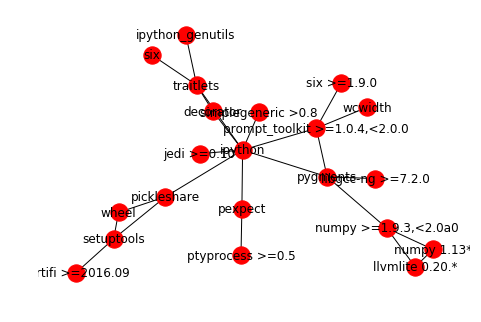
\includegraphics[width=0.5\textwidth , height=0.3\textheight]{dependency.png}
\caption{Dependency graph of the IPython Project.}
\end{figure}

The supply chain management concept what comes next to analyze the complex structure of the IPython project. We are going to analyze risk associated in consumers and suppliers relationships with the prediction of critical supplier in the IPython project. We evaluate three key parameters: number of dependencies, date of package release and version of package release of each library to predict the risk belonging to the particular supplier of the supply chain network.


\subsection {Results}

The preliminary results to analyze supply chain in IPython for different parameters is given below:  
\subsubsection{Number of Dependency}
We count the number of dependencies for each package. We examine the supply-chain risk utilizing the number of dependencies for the individual package. Following Table I shows the number of dependencies for some packages of the IPython. 

\begin{table} [h]
\begin{center}
\caption{Number of dependency packages}
\begin{tabular}{ |p{3.5cm}|p{3.5cm}| }
\hline
 Name of package & Number of dependency \\
 \hline
libgcc-ng  & 5\\
 \hline
pygments  & 3\\
    \hline
 numpy & 2\\
 \hline
 traitlets & 2\\

    \hline
   
\end{tabular}

\end{center}
\end{table}

In the table, last tier supplier package libgcc.ng has higher number of dependencies than other packages and which is pretty sure that it may add vulnerability on the IPython project.
\subsubsection{Date of Release}
This parameter is extracted from the file name LICENSE.txt of each package and used to compute the date of release. It provides the information whether supply chain network uses an updated version of packages or not. Following Table II shows some recent release packages of IPython.   

\begin{table} [h]
\begin{center}
\caption{Date of packages release}
\begin{tabular}{ |p{3.5cm}|p{3.5cm}| }
\hline
 Name of package&Release date \\
 \hline
mkl\_fft & 2017\\
 \hline
numpy & 2005-2017\\
    \hline
 pygments & 2006-2017\\
 \hline
 parso & 2015 \\

    \hline
   
\end{tabular}

\end{center}
\end{table}

From this data, supply chain network helps to tell about date of release of each package and can warn project that may have to face unpredictable issues.
\subsubsection{Version of Release}
This parameter provides the release version of each package and used to figure out whether they are the latest version or not. The version of some packages of IPython is listed in Table III below.  

\begin{table} [h]
\begin{center}
\caption{Release version of packages}
\begin{tabular}{ |p{3.5cm}|p{3.5cm}| }
\hline
 Name of package&Version \\
 \hline
libgcc-ng  & 3.2.1\\
 \hline
pygments  & 2.2.0\\
    \hline
 numpy &1.14.3\\
 \hline
 traitlets & 4.3.2\\

    \hline
   
\end{tabular}

\end{center}
\end{table}



From above evaluation, it is clear that the package libgcc-ng has more dependencies than other packages and hence more critical package in the supply chain system of the IPython project. The other packages has less than 50\% dependencies compare to libgcc-ng in the dependency network. This means any updates and crash in these packages have less impact rather than any updates happened only in the libgcc-ng package.




\section{Discussion -0.5}

Summarize the Opportunities and Challenges 



\section*{Acknowledgment}

\bibliographystyle{abbrv}
\bibliography{main}
\end{document}
